\documentclass[a4paper]{article}
\usepackage{caption}
\usepackage{fancyhdr}
\usepackage[usenames, dvipsnames]{xcolor}
\usepackage{graphicx,hyperref,amsmath,float,subfigure,soul}
\usepackage[top=3cm,bottom=3cm,left=3cm,right=3cm]{geometry}
\hypersetup{
	colorlinks,
	citecolor=black,
	filecolor=black,
	linkcolor=black,
	urlcolor=black
}
\newcommand{\HRule}{\rule{\linewidth}{0.5mm}}
\pagestyle{fancy}
\lfoot{\small \color{gray}Tom Peerdeman - 10266186}
\cfoot{\thepage}
\rfoot{\small \color{gray}Ren\'e Aparicio Sa\'ez - 10214054}
\lhead{\small \color{gray} CUDA}
\begin{document}
	\begin{titlepage}
	\begin{center}
		\textsc{\Large Concurrency \& Parallel Programming}\\[0.5cm]
		\HRule \\[0,4cm]
		\textsc{\huge \bfseries CUDA}
		\HRule \\[8cm]
		\begin{minipage}{0.4\textwidth}
			\begin{flushleft}\large
				\emph{Auteurs: Tom Peerdeman \& Ren\'e Aparicio Saez}\\
			\end{flushleft}
		\end{minipage}
		\begin{minipage}{0.4\textwidth}
			\begin{flushright}\large
			\emph{Datum: 08-12-2012\\\hspace{1cm}}\\
			\end{flushright}
		\end{minipage}
	\end{center}
	\end{titlepage}

\section{Assignment 6.1 - Wave simulation}
  
	\subsection{Results}
		For accuracy all the experiments are ran on the same node after each other, the node was first warmed up by running the program a couple times.\\
		\\
		In table \ref{table:iChange1000} we can see the results of 10 runs with different i\_max settings and a t\_max of 1000.
		In previous experiments we discarded the highest and lowest value, this is not realy useful in these test series since the test results are too close to each other.\\
		\\
		We can see from the average value's in the table that the increase in calculation point leads to a decreased average run time.
		This is a suprising result, since we would expect that more calculations leads to a longer execution time.
		The decrease in time could be caused by better utilizing the GPU's recources.
		A GPU works best if it has multiple threads scheduled for one ALU, in the case of multiple threads it can swith very fast between threads and pipeline the instruction's.
		If we would have just one thread per ALU, the threadss instruction's would be scheduled as well, but when a dependency exists a lot of no-op instruction's have to be inserted.
		With multiple threads these no-op instructions could be replaced by useful instructions of other threads.
		
		\begin{table}[H]
			\caption{Calculation times of the CUDA driven wave simulation in ms using a t\_max of 1000.}
			\label{table:iChange1000}
			\begin{center}
				\begin{tabular}{| c | c | c | c | c |}
					\hline
					\multicolumn{5}{|l|}{t\_max = 1000, 512 threads per block}\\
					\hline
					i=1e3 & i=1e4 & i=1e5 & i=1e6 & i=1e7\\ 
					\hline
					4,95 & 5,05 & 4,94 & 3,36 & 3,32\\ 
					\hline
					3,41 & 3,57 & 3,32 & 3,35 & 3,31\\ 
					\hline
					3,42 & 3,54 & 3,34 & 3,36 & 3,3\\ 
					\hline
					4,91 & 5,05 & 3,24 & 3,35 & 3,31\\ 
					\hline
					3,49 & 3,47 & 3,3 & 3,37 & 3,3\\ 
					\hline
					4,91 & 3,49 & 3,34 & 3,36 & 3,31\\ 
					\hline
					4,91 & 3,5 & 4,89 & 3,41 & 3,32\\ 
					\hline
					4,93 & 5,02 & 4,94 & 3,37 & 3,3\\ 
					\hline
					3,46 & 5,06 & 4,95 & 3,38 & 3,31\\ 
					\hline
					4,93 & 5,01 & 4,92 & 3,34 & 3,3\\ 
					\hline
					\multicolumn{5}{|l|}{Average over 10 runs:}\\
					\hline
					4,332 & 4,276 & 4,118 & 3,365 & 3,308\\ 
					\hline
				\end{tabular}
			\end{center}
		\end{table}
		
		\noindent Since all the buffers have to be rotated after each time step all the calculating threads have to synchronize after each time step.
		We could therefore say that the timesteps are calculated sequentially.
		If we would decrease the amount of time steps by a factor of 10, we would expext a time that is 10 times lower.
		In table \ref{table:iChange100} the reduction by a factor 10 is executed.
		We can see that the increase of time is not 10, also the speed increase decreases with a larger i\_max.
		The decrease in speed increase can be explained by the discovery we made in the begin: more calculation points gives a smaller caluclation time.
		The increase not being 10 could be explained by utilizing caches more in de later time steps.
		
		\begin{table}[H]
			\caption{Calculation times of the CUDA driven wave simulation in $\mu$s using a t\_max of 100.}
			\label{table:iChange100}
			\begin{center}
				\begin{tabular}{| c | c | c | c | c |}
					\hline
					\multicolumn{5}{|l|}{t\_max = 100, 512 threads per block}\\
					\hline
					i=1e3 & i=1e4 & i=1e5 & i=1e6 & i=1e7\\ 
					\hline
					529 & 555 & 374 & 392 & 399\\ 
					\hline
					391 & 383 & 373 & 397 & 406\\ 
					\hline
					534 & 554 & 367 & 405 & 396\\ 
					\hline
					530 & 397 & 541 & 391 & 574\\ 
					\hline
					539 & 540 & 542 & 403 & 395\\ 
					\hline
					388 & 395 & 373 & 396 & 383\\ 
					\hline
					538 & 384 & 542 & 404 & 383\\ 
					\hline
					379 & 387 & 538 & 396 & 399\\ 
					\hline
					382 & 554 & 379 & 395 & 392\\ 
					\hline
					527 & 545 & 375 & 590 & 386\\ 
					\hline
					\multicolumn{5}{|l|}{Average over 10 runs:}\\
					\hline
					473,7 & 469,4 & 440,4 & 416,9 & 411,3\\ 
					\hline
					\multicolumn{5}{|l|}{Speed increase vs t\_max = 1000:}\\
					\hline
					9.15 & 9.11 & 9.35 & 8.07 & 8.04\\
					\hline
				\end{tabular}
			\end{center}
		\end{table}
		
	\subsection{Speed comparison}
		If we compare our CUDA implementation to the previous implementations based on Threads, MPI and openMP, we can see in table \ref{table:speedComparison} that out CUDA implementation is by far the fastest.
		This result isn't suprising, the GTX 480 used has 15 SM units.
		Each of this SM units contain 32 ALU's, so in theory we can run 15 * 32 = 480 threads at the same time.
		The next fastest is the MPI implementation with 8 nodes running each 8 processes, this counts up as 64 processes/threads.
		Lets say this implementation scales up perfectly by time, so if we use 7.5 times more threads/processes the time would be 7.5 times lower.
		The implementation would use 480 threads/processes then and the time would be 16.0187 ms.
		This time would still be almost 5 times slower than the CUDA implementation, while using the same amount of threads.\\
		\\
		The sequential implementation in table \ref{table:speedComparison} is given by the pThreads implementation using 1 thread.
		This method is truly sequential since it is executed by 1 thread, but the timing also counts some overhead given by the pThreads.
		Given this we should keep in mind that a pure sequential implementation would be slightly faster than the given time under sequential in table \ref{table:speedComparison}.
		Keeping this in mind, we see that the CUDA implementation is over a thousand times faster than the (almost) sequential implementation.
		
		\begin{table}[H]
			\caption{Speed comparison between pthreads, MPI, openMP and CUDA, t\_max = 1000, i\_max = 1e6.}
			\label{table:speedComparison}
			\begin{center}
				\begin{tabular}{| l | c | c |}
					\hline
					Method & Average time (ms) & CUDA speedup\\
					\hline
					CUDA - 512 threads per block & 3.365 & 1.0\\
					\hline
					MPI - 8 nodes with 8 processes each & 120.140 & 35.703\\
					\hline
					MPI - 8 nodes with 1 process each & 495.634 & 147.291\\
					\hline
					OpenMP - 8 threads - static scheduler & 661.320 & 196.529\\
					\hline
					pThreads - 8 threads & 677.751 & 201.412\\
					\hline
					MPI - 1 node 8 processes & 1186.726 & 352.667\\
					\hline
					pThreads - 1 thread / Sequential & 3788.914 & 1125.977\\
					\hline
				\end{tabular}
			\end{center}
		\end{table}
	
	
	
	\subsection{Block sizes}
		Running a program using CUDA requires to pass the amount of threads per block into the program, in the wave simulation the number of blocks also depends on the number of threads per block.
		In table \ref{table:blockSizes} the wave simulation was ran using different amounts of threads per block.
		As we can see the amount of threads does not influence the calculation time.
		All the result do not differentiate much from each other, certainly not if we consider some margin of error in the results.
	
		\begin{table}[H]
			\caption{Calculation times of the CUDA driven wave simulation using different amounts of threads per block.}
			\label{table:blockSizes}
			\begin{center}
				\begin{tabular}{| c | c | c | c | c | c | c |}
					\hline
					16 & 32 & 64 & 128 & 256 & 512 & 1024\\ 
					\hline
					3,45 & 3,46 & 3,49 & 3,42 & 3,46 & 3,46 & 3,45\\ 
					\hline
					3,45 & 3,42 & 3,45 & 3,42 & 3,45 & 3,39 & 3,48\\ 
					\hline
					3,45 & 3,44 & 3,45 & 3,47 & 3,42 & 3,44 & 3,43\\ 
					\hline
					3,43 & 3,47 & 3,48 & 3,45 & 3,47 & 3,45 & 3,45\\ 
					\hline
					3,42 & 3,45 & 3,48 & 3,4 & 3,45 & 3,41 & 3,66\\ 
					\hline
					3,46 & 3,43 & 3,42 & 3,44 & 3,49 & 3,46 & 3,63\\ 
					\hline
					3,45 & 3,42 & 3,4 & 3,4 & 3,44 & 3,46 & 3,48\\ 
					\hline
					3,45 & 3,41 & 3,5 & 3,44 & 3,47 & 3,46 & 3,45\\ 
					\hline
					3,48 & 3,43 & 3,44 & 3,47 & 3,49 & 3,43 & 3,47\\ 
					\hline
					3,42 & 3,45 & 3,49 & 3,47 & 3,45 & 3,41 & 3,5\\ 
					\hline
					\multicolumn{7}{|l|}{Average over 10 runs:}\\
					\hline
					3,446 & 3,438 & 3,46 & 3,438 & 3,459 & 3,437 & 3,5\\ 
					\hline
				\end{tabular}
			\end{center}
		\end{table}
		
	
	\subsection{Results comparison}
		In figure \ref{fig:1000MPI} we can see the result of the wave simulation using the MPI implementation.
		If we compare this figure to the CUDA result in figure \ref{fig:1000CUDA} we see that they don't differ very much.
		\begin{figure}[H]
			\begin{center}
				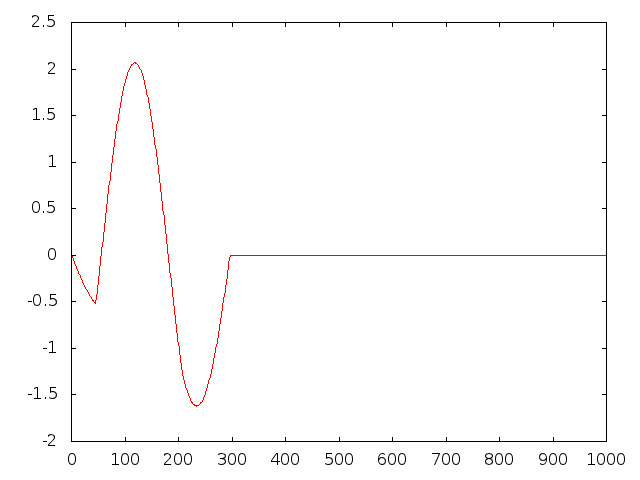
\includegraphics[scale=0.5]{1000MPI}
			\end{center}
			\caption{Result of running the wave simulation using MPI with i\_max = 1000 and t\_max = 100.}
			\label{fig:1000MPI}
		\end{figure}
		
		\begin{figure}[H]
			\begin{center}
				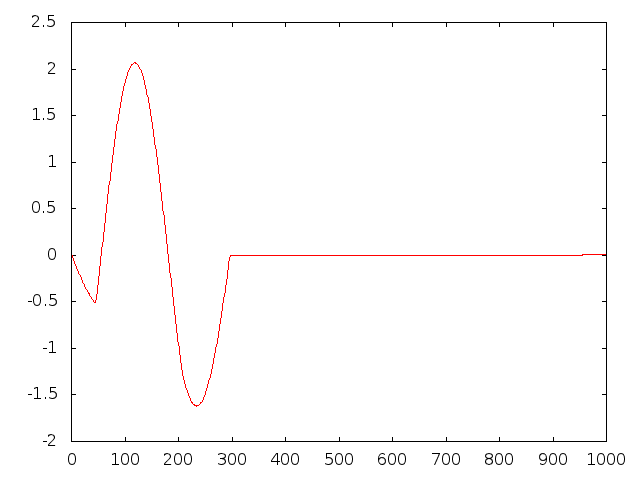
\includegraphics[scale=0.5]{1000CUDA}
			\end{center}
			\caption{Result of running the wave simulation using CUDA with i\_max = 1000 and t\_max = 100.}
			\label{fig:1000CUDA}
		\end{figure}
		
		\noindent The difference of results are therefore plotted in figure \ref{fig:resultsDiff}.
		We can see that the only differences lies in the begin and the end of the data.
		
		\begin{figure}[H]
			\begin{center}
				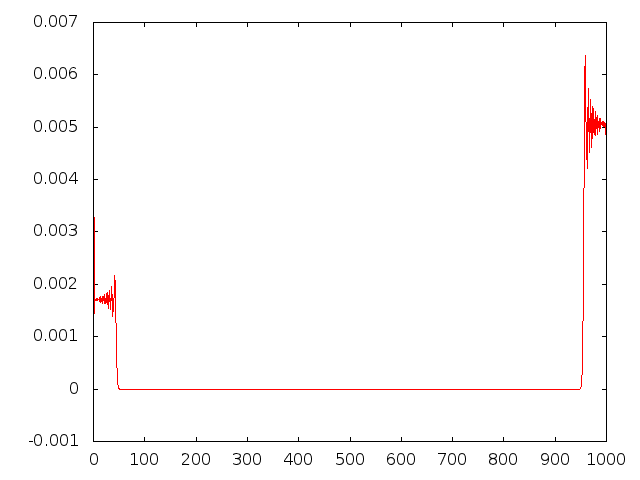
\includegraphics[scale=0.5]{results_diff}
			\end{center}
			\caption{Absolute difference in results of running the wave simulation using MPI and CUDA with i\_max = 1000 and t\_max = 100.}
			\label{fig:resultsDiff}
		\end{figure}
		
		\noindent These differences can be explained by the implementation of the handling of the edge values.
		The MPI implementation fixes the edge value's to zero each time step, the CUDA implementation simply ignores the edge values and doesn't do any calculations on it.
		The points next to the edge points also utilize the value of the edge points, so these will be different in the CUDA and MPI implementation.
		This error propagates to the next time step where the next to the next edge value is affected, this leads to the triangle shape from the edges.
		

	

\section{Assignment 6.2 - Parallel reduction}

\end{document}
